\documentclass[book.tex]{subfiles}
\begin{document}
This chapter describes the target hardware of Wolfenstein 3D. Each stage in the pipeline is detailed :
\begin{itemize} 
  \item CPU fasfasd fasdfasdf asfas asdf asdf asd fasf asdf sdf asf asf asf asf asdfsafasfasfasf a dsf asdf sdf 
  \item RAM
  \item Video
  \item Audio
  \item Inputs
\end{itemize}

\begin{figure}[!htb]
\centering
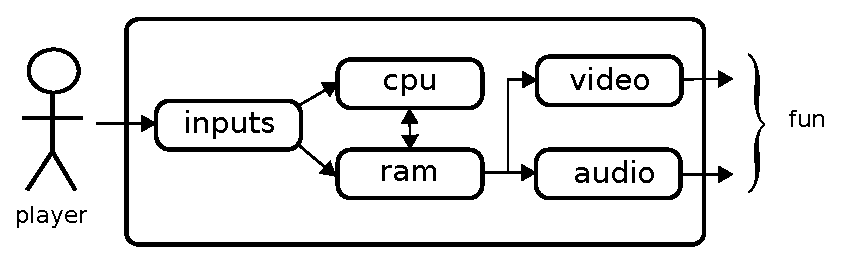
\includegraphics[scale=0.7]{../imgs/fun_pipeline.eps}
\caption{Fun pipeline.}
\label{fig:digraph}
\end{figure}
           

With a few exceptions, hardware mannufacturers had not embrased the game industry yet: Those machines were designed to display static images and crunch integers. Real-time 3D, fractions and smooth 60 fps animations were not part of the blueprints.

\section{CPU}
  \subsection{History}
  The ubiquitous manufacturer was Intel and its x86 line of microprocessors. Two other companies were also producing Intel clones: AMD and Cyrix but their mediocre performances denied then any significant market shares. Intel's 80286 processors from 1982 were dissapearing and were being replaced by their first 32bits processor: The i386 released in 1985. Moore's law was in full effect and the high end 386-DX 33Mhz was an obvious beast when plotten on a MIPs\footnote{Million Instructions per Second.} histogram  :

\definecolor{skyblue1}{rgb}{0.1,0.624,0.812}


\begin{figure}[!htb]
\centering
  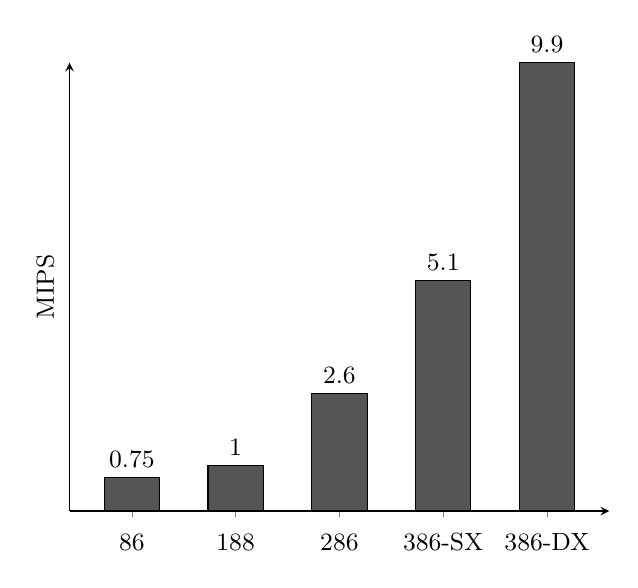
\begin{tikzpicture}[font=\small]
    \begin{axis}[
      ybar,
      bar width=20pt,
      ylabel={MIPS},
      ymin=0,
      ytick=\empty,
      xtick=data,
      axis x line=bottom,
      axis y line=left,
      enlarge x limits=0.15,
      symbolic x coords={86,188,286,386-SX,386-DX},
      xticklabel style={anchor=base,yshift=-\baselineskip},
      nodes near coords={\pgfmathprintnumber\pgfplotspointmeta}
    ]
      \addplot[fill={rgb:red,0.5;green,0.5;blue,0.5}] coordinates {
        (86,0.75)
        (188,1)
        (286,2.6)
        (386-SX,5.1)
        (386-DX,9.9)
      };
    \end{axis}
    
   \end{tikzpicture}
   \caption{Processor speeds comparaison.} \label{fig:mips}
 \end{figure}

Include comparaison with NES, C64 and Amiga  ?
 
 \textbf{\underline{Note :}} The huge performance difference between the 386-SX and the 386-DX is due to their bus width: The DX bus is twice as wide (32 bits) as the SX (16 bits) and therefore can retrieve data faster.
 \\

To keep things into perspective, a modern 2014 processor such as Intel Sandy Bridge operates at close to 30,000 Mips:

COMPARE WITH TODAY MIPS

  Wolfenstein 3D recommended configuration would end up being a 386 processor (while still being playable on a 286). It may be surprising after descriving how powerful
  But all that power was not useful for a 3D engine and it had to do with how calculations are done in a 3D game. In order to do trigonometry, operations need
  to keep track of fractions. Noawadays, developers are commonly using \emph{float} or 
  \emph{double} which are floating point types. Floating point are great, since they keep track of the fractionnal part of a number and the operations on it:


  But there was a huge problem with the hardware of 1992: CPU had no floating point unit. Which means that even though you could use floating point, those operations were emulated in software and therefore impossibly slow: Floating Point could not be used.

  Without the ability to do proper trigonometry, the perspective of building a 3D engine looked bleak.

  \subsection{Floating Point}
  \subsection{Fixed Point}

\section{RAM}
  386 very powerful (run linux 4GB, MMU) buy a major obstable stood between the programmer and the machine. It was the operating system and its name was DOS 4.0.
  \\
  \subsection{DOS limitations}

  \subsection{Infamous 16 bits segmented RAM}

\begin{verbatim}
    0110 1000 1000 0111 0000  Segment, 16 bits shifted 4 bits left  
  +      0011 0100 1010 1001  Offet,   16 bits
============================
    0110 1011 1101 0001 1001  Address, 20 bits
\end{verbatim}

  \subsection{Extended Memory}
  
\section{Video}
  \subsection{VGA Architecture}
  \subsection{VGA setup}
  \subsection{VGA Programming}
  \subsection{VGA Mode Y}
\section{Audio}
  \subsection{Speaker}
  \subsection{Ad Lib}
  \subsection{Sound Blaster}

\section{Inputs}

\end{document}




